\textcolor{black}{\section{Resultados y Análisis}}

\section{Cristal de NaCl 1 (mediciones nuestras)}
\noindent

\section{Cristal de NaCl 2 (base de datos)} %%%% ES EL "Cristal 1" EN EL EXCEL
\noindent En la Figura \ref{fig:GRAFICA_CRISTAL-1} se pudo observar una tendencia creciente sin relación alguna con la ley de Bragg, por lo que solo se trabajó con el primer pico (correspopndiende al primer orden de refracción, $n=1$). Este pico correspondió a un ángulo (en escala $2\theta$) de $35^\circ \pm 0.5^\circ$, por lo que el entonces el valor con el que se trabajó en la ley de Bragg fue de

\begin{equation}\label{eq:THETA-CRISTAL-1}
	\theta = 17.5^\circ \pm 0.25^\circ.
\end{equation}

Se sustituyó dicho valor (Ecuación \ref{eq:THETA-CRISTAL-1}) en la ley de bragg y se obtuvo una distancia interplanar de

\begin{equation}\label{eq:d-CRISTAL-1}
	d = 2.56\text{\AA} \pm 0.04\text{\AA}.
\end{equation}

Se comparó con los valores tabulados para NaCl \cite{NaCl-Teorico} y se encontró que la reflexión permitida más cercana corresponde a la familia ($200$), para la cual $d_{200}=2.82\,\text{\AA}$. Sin embargo, el valor experimental presenta una diferencia del $-9.22\%$ por lo que no resulta compatible con la Ecuación \ref{eq:d-CRISTAL-1} dentro de la incertidumbre experimental estimada.

\begin{figure}%[H]
	\centering
	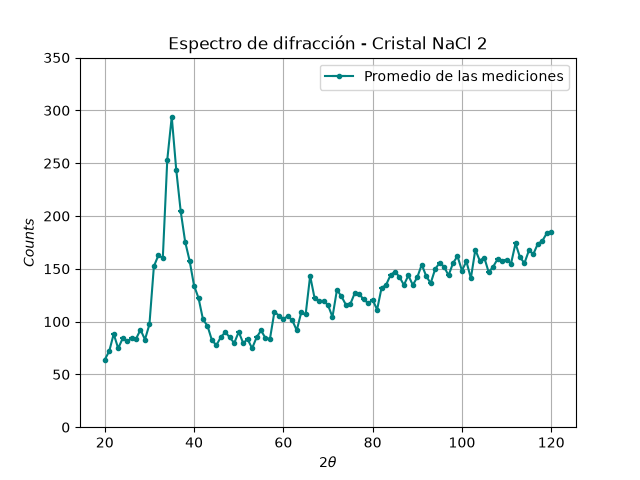
\includegraphics[scale=0.6]{figs/GRAFICA_CRISTAL-1.png}
	\caption{Conteos promedio registrados con respecto al ángulo de incidencia de rayos x para un cristal de NaCl.}
	\label{fig:GRAFICA_CRISTAL-1}
\end{figure}

\section{Cristal de NaCl 3 (base de datos)} %%%% ES EL "Cristal 4" EN EL EXCEL
\noindent

\section{Cristal de KCl (base de datos)} %%%% ES EL "Cristal 3" EN EL EXCEL
\noindent En la Figura \ref{fig:GRAFICA_CRISTAL-3} se pudo observar una tendencia creciente sin relación alguna con la ley de Bragg, por lo que solo se trabajó con el primer pico (correspopndiende al primer orden de refracción, $n=1$). Este pico correspondió a un ángulo (en escala $2\theta$) de $33^\circ \pm 0.5^\circ$, por lo que el entonces el valor con el que se trabajó en la ley de Bragg fue de

\begin{equation}\label{eq:THETA-CRISTAL-3}
	\theta = 16.5^\circ \pm 0.25^\circ.
\end{equation}

Se sustituyó dicho valor (Ecuación \ref{eq:THETA-CRISTAL-3}) en la ley de bragg y se obtuvo una distancia interplanar de

\begin{equation}\label{eq:d-CRISTAL-3}
	d = 2.71\text{\AA} \pm 0.08\text{\AA}.
\end{equation}

Se comparó con los valores tabulados para NaCl \cite{KCl-Teorico} y se encontró que la reflexión permitida más cercana corresponde a la familia ($200$), para la cual $d_{200}=3.14\,\text{\AA}$. Sin embargo, el valor experimental presenta una diferencia de $-13.69\%$ por lo que no resulta compatible con la Ecuación \ref{eq:d-CRISTAL-3} dentro de la incertidumbre experimental estimada.

\begin{figure}%[H]
	\centering
	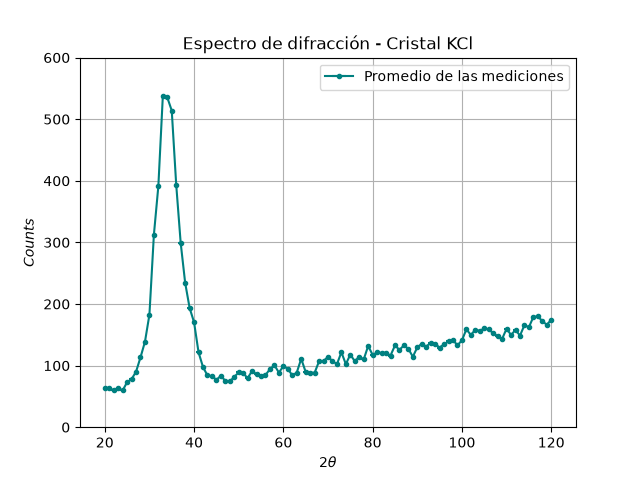
\includegraphics[scale=0.6]{figs/GRAFICA_CRISTAL-3.png}
	\caption{Conteos promedio registrados con respecto al ángulo de incidencia de rayos x para un cristal de KCl.}
	\label{fig:GRAFICA_CRISTAL-3}
\end{figure}
